\chapter{Branch and Bound algorithm}
\section{Pseudocodice}
Fase di Branching

Fase di Pruning

I solver cercano di tagliare creare alberi più piccoli possibile, tagliando il più possibile

Branch-and-cut-and-Bound: I tagli vengono fatti dove vi sono disuglianze valide

Lavora con una lista di L problemi LP→ Il problema LP di un nodo lo si chiamerà $N_k$ (k contatore di nodi esplorati) ed una soluzione ammissibile intera $\underline{x}$ (Incumbment solution) di valore LB=$-\infty$

\noindent \textbf{Pseudocodice:}

q=Numero di nodi totale

\begin{enumerate}
    \item \textbf{Step 0-INIT:} Fare il rilassamento contuinuo del problema ILP→$N_0$, inserire $N_0$ dentro la lista L; LB=$-\infty$ oppure al valore di una soluzione euristica → $\underline{x}=x_h$
    \item \textbf{Step 1-Termination check:} Se la lista L è vuota allora Z(ILP)=LB e l’incumbment solution è una soluzione ottima del problema LP
    \item \textbf{Step 2-Selezione del nodo di branching:} Selezionare un problema $LP(N_k)$ dalla lista L e cancellarlo dalla lista
    \item \textbf{Step 3-Bounding:} Risolvere il problema $LP(N_k)$, se è infeasable go to \textbf{step 1} [Prune by infeasability], altrimenti sia $\tilde{x}^k$ la soluzione ottima di $N_k$ e $z(N_k)$ Il valore della soluzione $\tilde{x}^n$
    \item \textbf{Step 4-Pruning:} 
    \begin{enumerate}
        \item Se $z(N_k) \leqslant LB$ go to \textbf{step 1} [Prune by bound]  (Non ci sono soluzioni migliori)
        \item Se $\tilde{x}^k$ non è intera go to \textbf{step 5}, altrimenti $LB=z(N_k)$ (Aggiorno incumbent solution), $\underline{x}=\tilde{x}^k$ go to \textbf{step 1} [Prune by integrity]
        \item Cancellare da L i nodi $z(N_k) \leqslant LB$
    \end{enumerate}
    \item \textbf{Step 5-Branching:} Da $N_k$ costruire un insieme di s problemi LP $N_{q+1}, N_{q+2}, …, N_{q+s}$ con la proprietà che tutte le soluzioni intere di $N_k$ siano nell’unione dei s problemi LP creati; Aggiungo $N_{q+1}, N_{q+2}, …, N_{q+s}$ alla lista L, q=q+s e go to \textbf{step 1}
\end{enumerate}

\dfn{Branching strategy: Binaria per alberi binari (s=2)}{
\begin{enumerate}
    \item Un nodo con un upperbound aggiuntivo sul valore di una variabile
    \item Un nodo con un lowerbound sul valore di una variabile
\end{enumerate}


$N_k=\tilde{x}^k$ frazionaria

Selezionare una variabile con un valore frazionario $\tilde{x}^k_j$
\begin{align*}
    \begin{array}{c}
        \Downarrow\\
        N_{q+1=N_k} \text{con} x_j \leqslant\lfloor \tilde{x}^k_j\rfloor
    \end{array}
    &
    \begin{array}{c}
        \Downarrow\\
        N_{q+2}=N_k \text{con} x_j \leqslant\lfloor \tilde{x}^k_j\rfloor +1
    \end{array}
\end{align*}
}

\textbf{Node selection strategy:}

Strategia con cui si scegliere l’ordine con cui trattare la lista L
\begin{enumerate}
    \item First-in-first-out: Bfs, migliora l’upperbound
    \begin{center}
        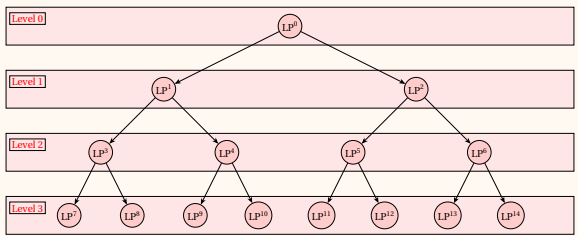
\includegraphics{bfs}
    \end{center}
    
    \item Last-in-first-out: Dfs, migliora l’incumbent solution
    \begin{center}
        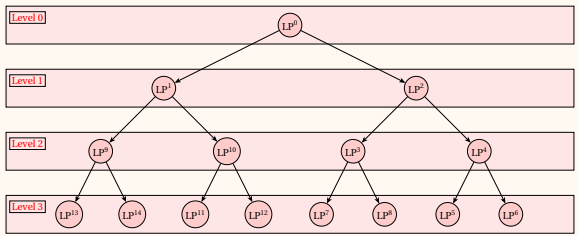
\includegraphics{dfs}
    \end{center}
\end{enumerate}

Livello Branching di un nodo $N_k$ → Numero di variabili con cui ho fatto branching

Sia $I(\alpha)$ l’insieme di tutti i nodi a profondità $\alpha$:
$z(ILP)\leqslant \underset{k\ \in\ I(\alpha)}{(z(N_k))}$

\textbf{Numero di nodi di un albero di branching}

In un albero generico con q nodi per livello abbiamo: 
\[
\sum_{k=0}^{n-1} q^k=\frac{q^n-1}{q-1}
\]
\begin{myproof}
    \[
    \begin{array}{c}
        \text{Base con n=1}\\
        \sum^0_{K=0}q^k\Rightarrow q^0 = 1= \frac{q^1-1}{q-1}=1\\
        \text{Caso induttivo:}\\
        \sum_{k=0}^{n+1-1} q^k=\sum_{k=0}^{n-1}\\
         q^k+q^n=\frac{q^n-1}{q-1}+q^n=\frac{q^n-1+q^{n+1}-q^n}{q-1}=\frac{q^{n+1}-1}{q-1}
    \end{array}
    \]
\end{myproof}

Il numero totale di nodi è $O(q^n)$ → per gli alberi binari è $O(2^n)$,
 la complessità nel caso peggiore del bound è esponenziale

\ex{Esempio da formulazione ILP}{

Se tutti i coefficienti della funzione obiettivo sono interi: 

\[
\begin{aligned}
    Max\ & x_1& +x_2 &\\& -x_1&+x_2 &\leq 2 \\& 8 x_1&+2x_2 &\leq 19 \\& x_1&, x_2 & \in \mathbb{Z}_{+}
\end{aligned} \\LP_0\ x_1,x_2 \geqslant 0\\  
\]

$z(ILP)\leqslant\lfloor Z(LP)\rfloor$

\begin{center}
    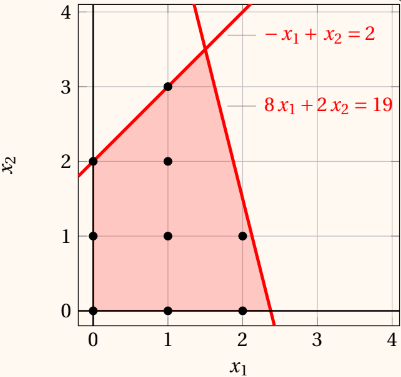
\includegraphics[height=3cm]{bb1}
\end{center}

\[
\tilde{x}_1=\frac{3}{2}, \quad \tilde{x}_2=\frac{7} \quad{2}z(\mathrm{LP})=5\\\underline{x}_1=\left\lfloor\frac{3}{2}\right\rfloor=1, \quad \underline{x}_2=\left\lfloor\frac{7}{2}\right\rfloor=3\\\underline{z}=1+3=4 \leq z\left(\text { ILP }_{\mathrm{KP}}\right)
\]

Creo due Lp con 2 condizioni: $\leqslant 1$ e $\geqslant2$ togliendo la parte non intera

\[
 \begin{aligned}Max\ & x_1& +x_2 &\\& -x_1&+x_2 &\leq 2 \\& 8 x_1&+2x_2 &\leq 19 \\ &x_1 && \leqslant 1\\& x_1&, x_2 & \in \mathbb{Z}_{+}\end{aligned} 
\]

$$
\tilde{x}_1=1, \quad \tilde{x}_2=3 \quad z(LP_1)=4 \quad \textbf{\textbf{Intera}}
$$
\begin{center}
    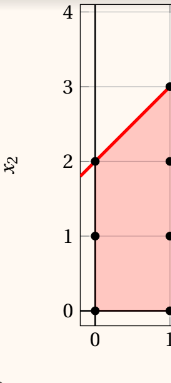
\includegraphics[height=3cm]{bb2}
\end{center}

\[
 \begin{aligned}Max\ & x_1& +x_2 &\\& -x_1&+x_2 &\leq 2 \\& 8 x_1&+2x_2 &\leq 19 \\&& x_2 & \geqslant 2\\& x_1&, x_2 & \in \mathbb{Z}_{+}\end{aligned} 
\]

$$
\tilde{x}_1=2, \quad \tilde{x}_2=\frac{3}{2} \quad z(LP_1)=\frac{7}{2} \quad \text{\textbf{Ramo Potato}}
$$
\begin{center}
    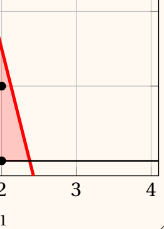
\includegraphics[height=3cm]{bb3}
\end{center}

}
